%        File: report.tex
%     Created: Sun Feb 21 08:00 AM 2016 E
% Last Change: Sun Feb 21 08:00 AM 2016 E
%
\documentclass[a4paper]{report}

\usepackage{mathtools} 
\usepackage{amsmath}
\usepackage{amssymb}
\usepackage{newlfont}
\usepackage{caption}
\usepackage{subcaption}
\usepackage{titlesec}
\usepackage{graphicx}
\usepackage{empheq}

\title{Written Preliminary Exam \#1 \break
       Prepared by Dr. Hassan}

\author{ Kyle B. Thompson }

\begin{document}
\maketitle

\begin{enumerate}
  \item Constant density flow and incompressible flow are two different things.
    Constant density implies that a fluid(s) density is constant, but capable of
    changing (through compression or expansion), whereas incompressible implies
    the fluid(s) density is incapable of changing but that the density in the
    flow is not constant.  A good example from the MAE 560 course to distinguish
    the two is stagnant air in a room, versus an oil/water mixture.  Stagnant
    air in a room is at constant density, but is certainly capable of both
    compression or expansion; therefore, it is a constant density flow, but not
    incompressible.  An oil/water mixture is not constant density.  As
    illustrated in figure \ref{fig:incompressible},the
    water and oil are different fluids with different densities, but the fluids
    are incompressible because both the water and oil are not capable of
    compression or expansion (at least in a practical sense); therefore, it not
    a constant density flow, but is incompressible.

    \begin{figure}[h]
      \centering
      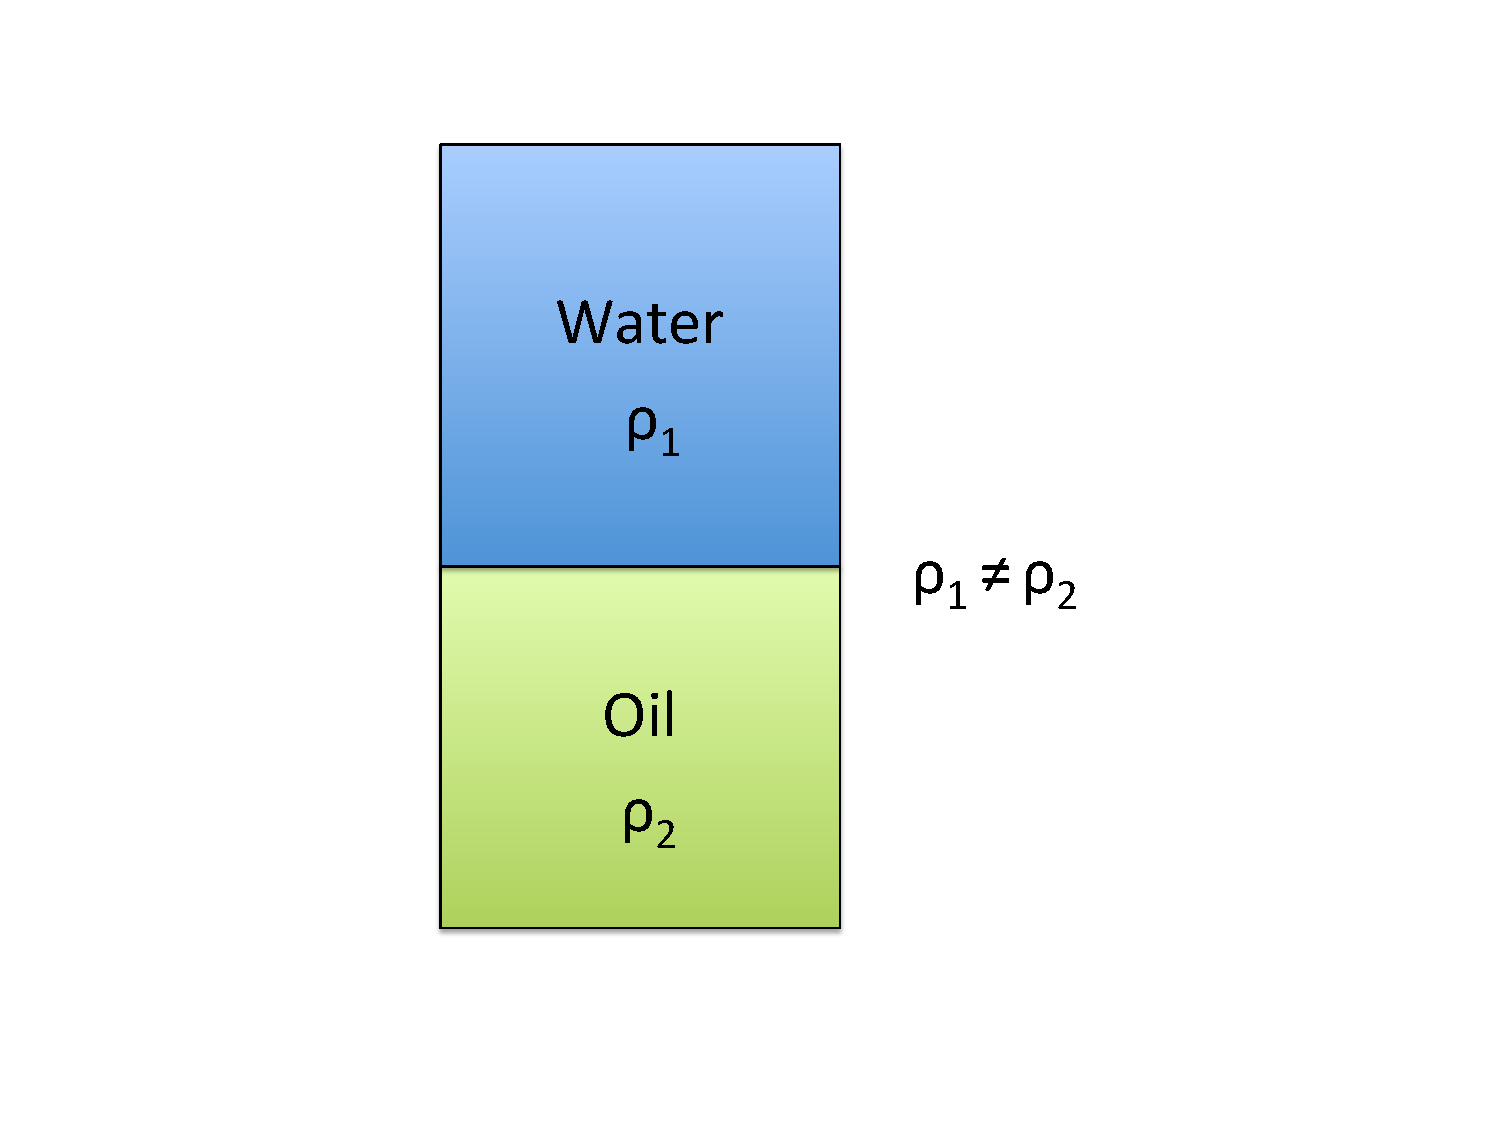
\includegraphics[width=0.8\textwidth,trim={0 2cm 0 2cm},clip]{oil_water_fig}
      \caption{Incompressible Fluid Flow Example}
      \label{fig:incompressible}
    \end{figure}

  \item There are many ways to derive an expression for change in entropy.
    From a statistical mechanics perspective, we can derive a function for
    entropy that is based upon the partition function, $Q$.

\end{enumerate}

\end{document}


